\subsection{Recurrent neural network}

Humans don’t start their thinking from scratch every second. As you read this essay, you understand each word based on your understanding of previous words. You don’t throw everything away and start thinking from scratch again. Your thoughts have persistence.

Traditional neural networks can’t do this, and it seems like a major shortcoming. For example, imagine you want to classify what kind of event is happening at every point in a movie. It’s unclear how a traditional neural network could use its reasoning about previous events in the film to inform later ones.

Recurrent neural networks address this issue. They are networks with loops in them, allowing information to persist.

\begin{figure}[H]
    \centering
    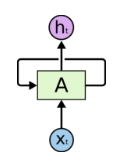
\includegraphics[width=2in]{images/rnn.png}
    \caption{Recurrent Neural Networks with loops.}
    \label{fig:rnnRoll}
\end{figure}

In the above diagram, a chunk of neural network, $A$, looks at some input $x_t$ and outputs a value $h_t$. A loop allows information to be passed from one step of the network to the next.

These loops make recurrent neural networks seem kind of mysterious. However, if you think a bit more, it turns out that they aren’t all that different than a normal neural network. A recurrent neural network can be thought of as multiple copies of the same network, each passing a message to a successor. Consider what happens if we unroll the loop:

\begin{figure}[H]
    \centering
    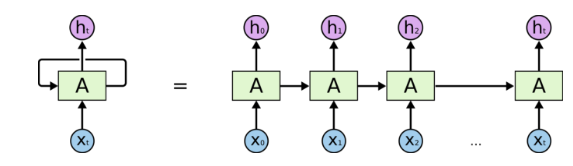
\includegraphics[width=6.5in]{images/rnnUnroll.png}
    \caption{Unrolled recurrent neural network.}
    \label{fig:rnnUnroll}
\end{figure}

This chain-like nature reveals that recurrent neural networks are intimately related to sequences and lists. For such data, they are the natural architecture of neural network.

And they certainly are used! In the last few years, there have been incredible success applying RNNs to a variety of problems: speech recognition, language modeling, translation, image captioning… The list goes on.

Over the years researchers have developed more sophisticated types of RNNs to deal with some of the shortcomings of the vanilla RNN model. I want this section to serve as a brief overview so that you are familiar with the taxonomy of models.

\subsubsection{Bidirectional RNNs}

Bidirectional recurrent neural networks(RNN) are really just putting two independent RNNs together. The input sequence is fed in normal time order for one network, and in reverse time order for another. The outputs of the two networks are usually concatenated at each time step, though there are other options, e.g. summation.

\begin{figure}[H]
    \centering
    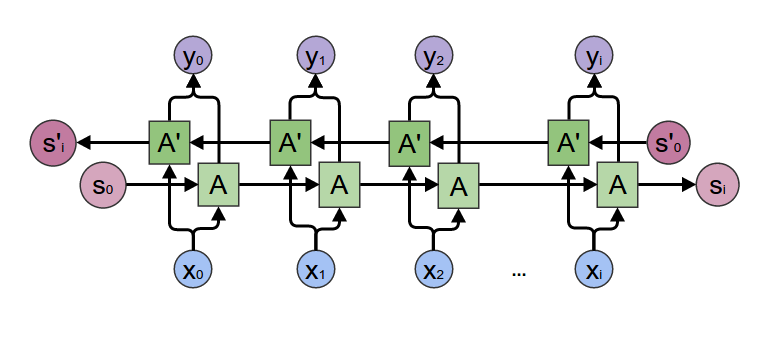
\includegraphics[width=6.5in]{images/bidirectionalRNN.png}
    \caption{General Structure of Bidirectional Recurrent Neural Networks.}
    \label{fig:bidirectionalRNN}
\end{figure}

This structure allows the networks to have both backward and forward information about the sequence at every time step.

They're often used when we’re trying to make predictions in a sequence. For example, in voice recognition, we might wish to predict a phenome for every time step in an audio segment, based on past context.

\subsubsection{Deep (Bidirectional) RNNs}

They're similar to Bidirectional RNNs, only that we now have multiple layers per time step. In practice this gives us a higher learning capacity (but we also need a lot of training data).

\subsubsection{LSTM networks}

One of the appeals of RNNs is the idea that they might be able to connect previous information to the present task. That work such as using previous video frames might inform the understanding of the present frame. If RNNs could do this, they’d be extremely useful. But can they? It depends.

Sometimes, to perform the present task, we only need to look at recent information. For example, consider a language model trying to predict the next word based on the previous ones. We don’t need any further context if we are trying to predict the last word in “the clouds are in the sky,”. – it’s pretty obvious the next word is going to be sky. In such cases, where the gap between the relevant information and the place that it’s needed is small, RNNs can learn to use the past information.


\begin{figure}[H]
    \centering
    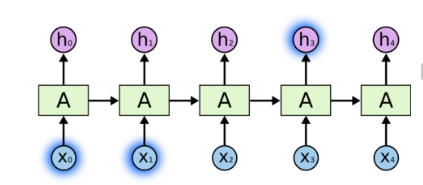
\includegraphics[width=4.5in]{images/rnnWhatWeNeed.png}
    \caption{Graphics representation for connecting informations}
\end{figure}


But there are also cases where we need more context. Consider trying to predict the last word in the text “I grew up in France… I speak fluent French.” Recent information suggests that the next word is probably the name of a language, but we need the context of France, from further back if we want to narrow down which language. It’s entirely possible for the gap between the relevant information and the point where it is needed to become very large.

Unfortunately, as that gap grows, RNNs become unable to learn to connect the information.

\begin{figure}[H]
    \centering
    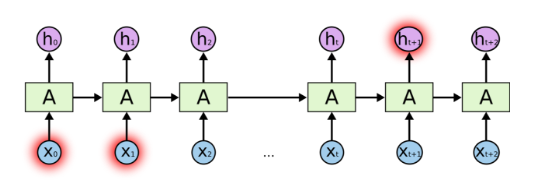
\includegraphics[width=6.5in]{images/rnnWhatWeNeedButCannot.png}
    \caption{Graphics representation for connecting informations, more data}
\end{figure}

In theory, RNNs are absolutely capable of handling such “long-term dependencies.” A human could carefully pick parameters for them to solve toy problems of this form. Sadly, in practice, RNNs don’t seem to be able to learn them. The problem was explored in depth by Hochreiter (1991) [German] and Bengio, et al. (1994), who found some pretty fundamental reasons why it might be difficult. \cite{lstm}

Thankfully, LSTMs don’t have this problem!

Long Short Term Memory networks – usually just called "LSTMs" – are a special kind of RNN, capable of learning long-term dependencies. They were introduced by Hochreiter \& Schmidhuber in 1997, and were refined and popularized by many people in following work. They work tremendously well on a large variety of problems, and are now widely used.

LSTMs are explicitly designed to avoid the long-term dependency problem. Remembering information for long periods of time is practically their default behavior, not something they struggle to learn!

All recurrent neural networks have the form of a chain of repeating modules of neural network. In standard RNNs, this repeating module will have a very simple structure, such as a single tanh layer.

\begin{figure}[H]
    \centering
    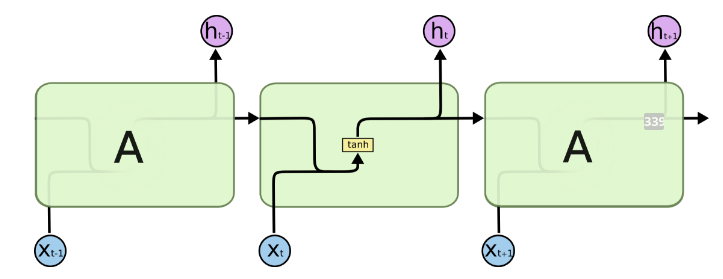
\includegraphics[width=6.5in]{images/rnnStandard.png}
    \caption{The repeating module in a standard RNN contains a single layer.}
\end{figure}

LSTMs also have this chain like structure, but the repeating module has a different structure. Instead of having a single neural network layer, there are four, interacting in a very special way.

\begin{figure}[H]
    \centering
    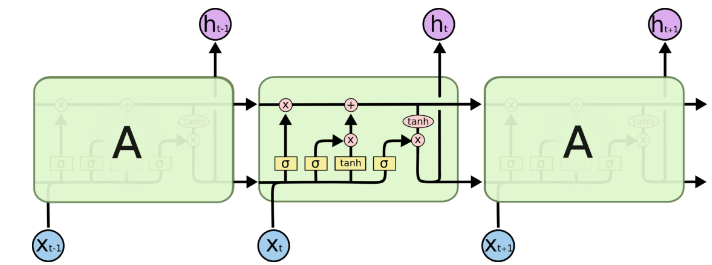
\includegraphics[width=6.5in]{images/lstm.png}
    \caption{The repeating module in an LSTM contains four interacting layers.}
\end{figure}
